\documentclass[a4paper,12pt]{report}
\usepackage{bbkproject}
\usepackage{lipsum}
\usepackage{amsthm}
\usepackage{amsmath}
\usepackage{graphicx}
\usepackage{amsfonts}
\usepackage{caption}
\usepackage{enumerate}% http://ctan.org/pkg/enumerate
\usepackage{seqsplit}

\usepackage{tabu}
%\subject{Mathematics}
%\degree{M.Sc.}
%\thesis{dissertation}

\theoremstyle{definition}
\newtheorem{definition}{Definition}[chapter]
\newtheorem{example}[definition]{Example}
\newtheorem{lemma}[definition]{Lemma}
%\setcounter{tocdepth}{1}

\begin{document}
\chapter*{Spring Progress Report}
\section*{Topology, Data and Manifold learning}
In the fields of statistics and machine learning, we are often preoccupied with learning an underlying manifold that minimizes some measure of error for this learning. The simplest example of this would be linear regression, where we seek to find a straight line (a space equivalent to $\mathbb{R}$, to describe the underlying relationship we assume to exist. The process of selecting an algorithm used for manifold learning or predictive modelling then depends on the family of manifold that underlies the data, with some algorithms or in particular algorithm hyper-parameters being more or less suited to any one given dataset. These questions of "families of manifolds" are dealt with- on one level at least- by discussions of their topology, and by extension topological inference methods on their observed data, such as that of persistent homology. In my dissertation, I wish to investigate the relationships between the inferred topological properties of data, to the topological properties of any underlying manifold structure, to the choice of models and hyper-parameters when attempting to learn relationships between different variables, and  in particular inferring the number of parameters or dimensions needed to separate, describe, encode or predict from any given dataset. Part of my research would involve the relationship between topological features of a dataset's underlying manifold and the topological features of the data itself arrived at through persistence methods

 \subsection*{Manifold Learning and Topology of Random Fields}
 When dealing with data, we are often concerned with reducing the dimensionality of it, especially when this dimension is very large; since in this case the data can be difficult to interpret, as well as computationally intractable. In this case we assume there is some underlying manifold of dimension lower than that of the space it is embedded in. There are a number of techniques we can use to attempt to encode data into a smaller number of sets of parameters, the most oldest example being principal component analysis \cite{pca} which describes an algorithm for building up a series of basis vectors for which the linear subspace they define minimizes the mean squared error of the point cloud from which they are generated, by taking the eigenvalue decomposition of the data's covariance matrix.
 
 
 Further to this, we may consider nonlinear methods. Autoencoders are a form of neural network that attempt to learn maps from the data to a lower dimensonal representation and then learn the identity map
  
 \begin{figure}[h]
\begin{center}
    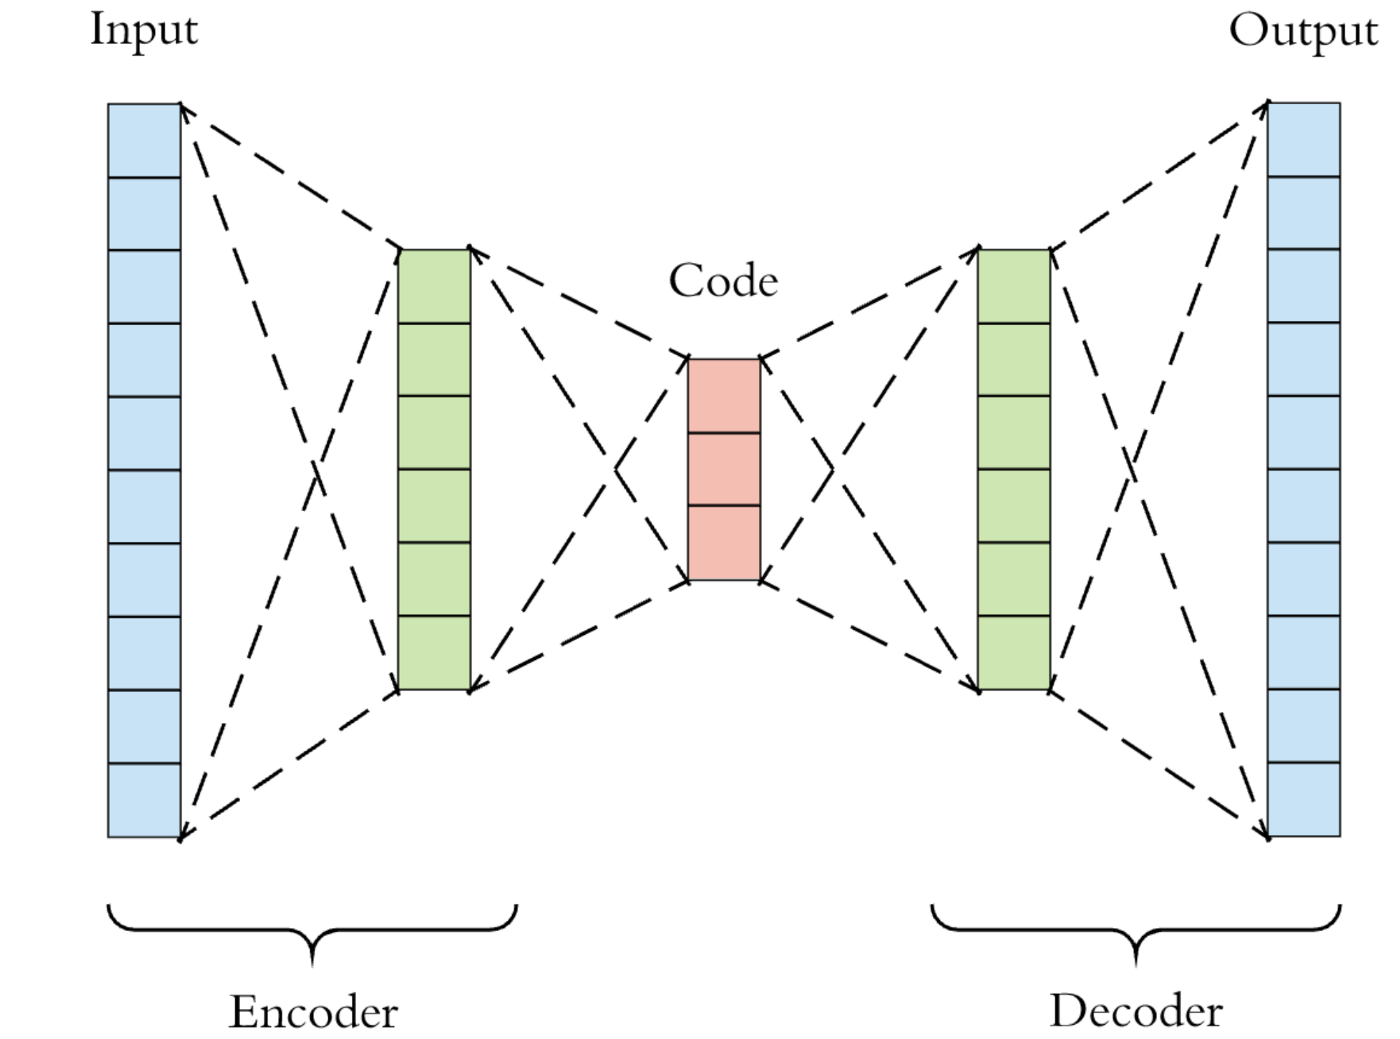
\includegraphics[width=0.5\textwidth]{autoencoder.png} 
    \caption{image taken from \cite{autoencoder} }
  \end{center}
 
 \end{figure}
This is arrived at by gradient descent methods. 

Not only do we care about reducing the dimensionality of our data, we may also wish to embed our data into higher dimensions for the purposes of classification.\cite{NNTop} describes the following important observation

 \begin{minipage}{0.5\textwidth}
 \begin{lemma}
 There does not exist a neural network with less than 3 hidden units that can solve the depicted classification problem
 \end{lemma}
 \end{minipage}\begin{minipage}{0.5\textwidth}
 \centering
 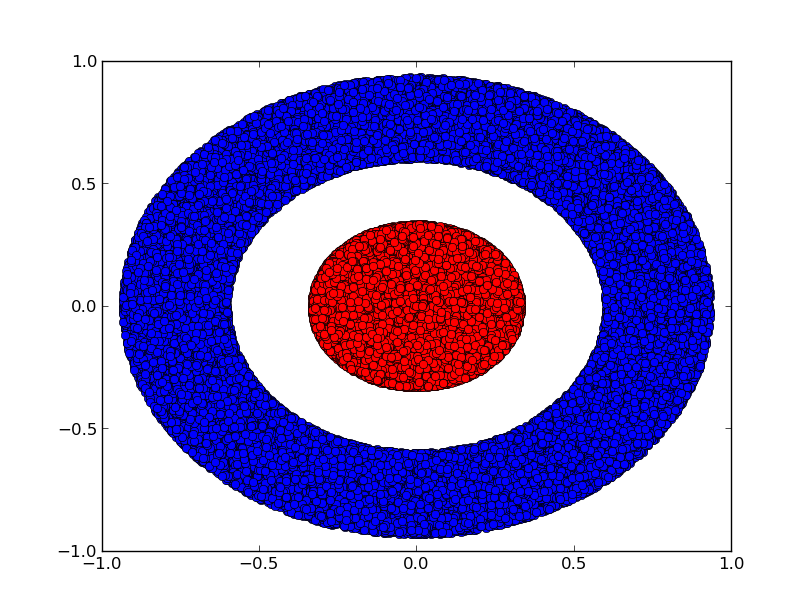
\includegraphics[width=0.7\textwidth]{topology_base.png}
 \end{minipage}
 as we can see, the layers of neural networks, and properties of other classification methods such as support vector machines, being homomorphisms (or being of rank 0) means the topology of the separating boundary has immediate implications for the types of methods that can be used, and certainly the complexity of those methods.
 \subsection*{Persistent Homology}
 The primary metholodology for computing the topology of a data's underlying manifold is through something called persistent homology. The motivation for this method is the wish to describe the topological features of a simplicial complex generated from a dataset at different scales, and to see which features {\em persist} across the most scales.
 
 \begin{definition}
 Let $f:X \rightarrow \mathbb{R}$ where $X$ a simplicial complex and $f$ is such that for $\sigma, \tau \in X$, if $\sigma < \tau$ then $f(\sigma)\leq f(\tau)$. Then the collection of sublevel sets $\{X(a): X(a) = f^{-1}((-\infty,a]), \; a \in \mathbb{R}\}$ forms a filtration by simplicial complex containment on this simplicial complex: $$\emptyset = X_0 \leq X_1 \leq \dots \leq X_n = X$$
 This induces homomorphisms on the simplicial homology groups of these simplicial complexes: when $i\leq j$,  $f^k_{i,j}: H_k(X_i)\rightarrow H_k(X_j)$. the images of these maps given a $p$ are called the $p^{\textrm{th}}$ persistent homology groups \cite{persistence}.
 
 We can construct one such face-nondecreasing function by considering the simplicial complex formed when joining $n$ points in a point cloud together with an $n$-simplex when their respective balls of radius $r$ intersect, then $f(\sigma) = r$  gives us the kind of function we need to do persistent homology. 
 \end{definition}
 \subsection*{Topology and Dimensionality of data}
 Once we have found topological features of data, especially high dimensional data, we can use this to choose the inference methods for this data. In \cite{NNTop} we see a discussion of how topological observations can be used to dictate neural network architecture, and it is this manner of discussion I wish to expand on in my dissertation.
 
 A simple example of this would be the largest dimensionality of a statistically significant hole, as arrived at through persistent homology, in the data could provide a lower bound for the dimensionality of the manifold from which it is sampled. In this dissertation I wish to establish the relationship that persistent homology of a point cloud has to any underlying manifold it is sampled from, expand on the kinds of dimensionality inferences we can make on the basis of topology, ascertain which kind of inference methods are best suited to which kinds of manifold learning, and prove some theorems which can be used to pre-select hyper parameters for the basis of this learning.
 
 \begin{thebibliography}{}
 \bibitem{pca} K. Pearson {\em On lines and planes of closest fit to systems of points in space} Philosophical Magazine 1901
 \bibitem{Lawrence} N. D. Lawrence {\em A Unifying Probabilistic Perspective for Spectral Dimensionality Reduction: Insights and New Models} JMLR, 2012
 \bibitem{persistence} H. Edelsbrunner, D. Letscher, and A. Zomorodian {\em Topological Persistence and Simplification} Discrete Comput Geom 2002
 \bibitem{NNTop} (Github User) Colah {\em Neural Networks, Manifolds, and Topology} 2014 https://colah.github.io/ posts/2014-03-NN-Manifolds-Topology/
 \bibitem{autoencoder} M. Stewart, {\em Comprehensive Introduction to Autoencoders} https://towardsdatascience.com/generating-images-with-autoencoders-77fd3a8dd368 2019
 \end{thebibliography}
\end{document}